%%% LaTeX Template: Article/Thesis/etc. with colored headings and special fonts
%%%
%%% Source: http://www.howtotex.com/
%%% Feel free to distribute this template, but please keep to referal to http://www.howtotex.com/ here.
%%% February 2011
%%%
%%% Modified January 2016 by CDM

%%%  Preamble
\documentclass[11pt,letterpaper]{article}
\usepackage[margin=1.0in]{geometry}
\usepackage[T1]{fontenc}
\usepackage[bitstream-charter]{mathdesign}
\usepackage[latin1]{inputenc}					
\usepackage{amsmath}						
\usepackage{xcolor}
\usepackage{cite}
\usepackage{hyphenat}
\usepackage{graphicx}
\usepackage{float}
\usepackage{subfigure}
\usepackage{sectsty}
\usepackage[compact]{titlesec} 
\usepackage[tablegrid]{vhistory}
\usepackage{pbox}
\allsectionsfont{\color{accentcolor}\scshape\selectfont}

%%% Definitions
\definecolor{accentcolor}{rgb}{0.0,0.0,0.5} 
\newcommand{\teamname}{LJCJ}
\newcommand{\productname}{UR20 Palletizer}
\newcommand{\coursename}{CSE 4317: Senior Design II}
\newcommand{\semester}{Spring 2025}
\newcommand{\docname}{Detailed Design Specification}
\newcommand{\department}{Department of Computer Science \& Engineering}
\newcommand{\university}{The University of Texas at Arlington}
\newcommand{\authors}{Luis Contreras \\ Joshua Dominguez \\ Christopher Gonzalez \\ Jasper Gustafson}

%%% Headers and footers
\usepackage{fancyhdr}
	\pagestyle{fancy}						% Enabling the custom headers/footers
\usepackage{lastpage}	
	% Header (empty)
	\lhead{}
	\chead{}
	\rhead{}
	% Footer
	\lfoot{\footnotesize \teamname \ - \semester}
	\cfoot{}
	\rfoot{\footnotesize page \thepage\ of \pageref{LastPage}}	% "Page 1 of 2"
	\renewcommand{\headrulewidth}{0.0pt}
	\renewcommand{\footrulewidth}{0.4pt}

%%% Change the abstract environment
\usepackage[runin]{abstract}			% runin option for a run-in title
%\setlength\absleftindent{30pt}			% left margin
%\setlength\absrightindent{30pt}		% right margin
\abslabeldelim{\quad}	
\setlength{\abstitleskip}{-10pt}
\renewcommand{\abstractname}{}
\renewcommand{\abstracttextfont}{\color{accentcolor} \small \slshape}	% slanted text

%%% Start of the document
\begin{document}

%%% Cover sheet
{\centering \huge \color{accentcolor} \sc \textbf{\department \\ \university} \par}
\vspace{1 in}
{\centering \huge \color{accentcolor} \sc \textbf{\docname \\ \coursename \\ \semester} \par}
\vspace{0.5 in}
\begin{figure}[h!]
	\centering
   	
\includegraphics[width=0.60\textwidth]{images/LJCJ.jpg}
\end{figure}
\vspace{0.5 in}
{\centering \huge \color{accentcolor} \sc \textbf{\teamname \\ \productname} \par}
\vspace{0.5 in}
{\centering \large \sc \textbf{\authors} \par}
\newpage


%\vspace{1 in}
%\centerline{January 13th, 2012}
%\newpage

%%% Revision History
\begin{versionhistory}
  	\vhEntry{0.1}{2.02.2025}{JG, JD, LC, CG}{Document creation}
        \vhEntry{0.2}{2.28.2025}{JG, JD, LC, CG}{Complete draft}

\end{versionhistory}
\newpage

%%% Table of contents
\setcounter{tocdepth}{2}
\tableofcontents
\newpage

%%% List of figures and tables (optional)
\listoffigures
\listoftables
\newpage

%%% Document sections
\section{Introduction}
Your introduction should provide a brief overview of the product concept and a reference to the requirement specification and architectural design documents in 1 or 2 paragraphs. The purpose is to provide the reader with the location of relevant background material that lead to the design details presented in this document.
\section{System Overview}
This section should reintroduce the full data flow diagram from the architectural specification, and discuss at a high level the purpose of each layer. You do not need to include a subsection for each layer, a 1 - 2 paragraph recap is sufficient.

\begin{figure}[h!]
	\centering
 	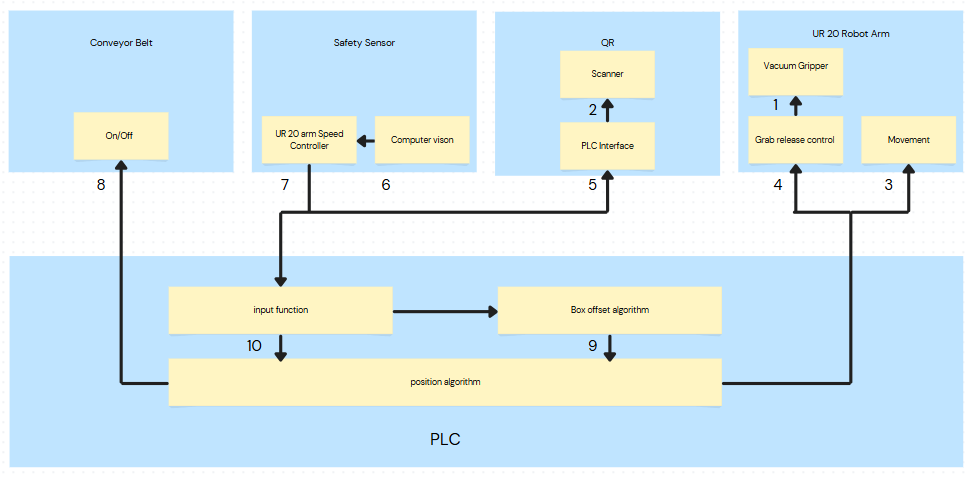
\includegraphics[width=0.90\textwidth]{images/data_flow}
 \caption{System architecture}
\end{figure}
\newpage
\section{UR 20 Robot Arm Layer Subsystems}
%% all subsystems insame format
The UR20 arm is the physical UR20 module. It can be controlled the a '3PE Teach Pendant' that allows touchscreen controls, or the Cobot URScript/Python URX library. This module covers the physical arm itself, the control mechanisms, and the gripper used for manipulating boxes.

\subsection{Layer Hardware}
The UR20 arm covers the UR20 arm, the control tablet, the control box, and gripper.

\subsection{Layer Operating System}
The Operating system used will be the UR PolycScope system that runs as the UR robots OS and programming interface.

\begin{figure}[h!]
	\centering
 	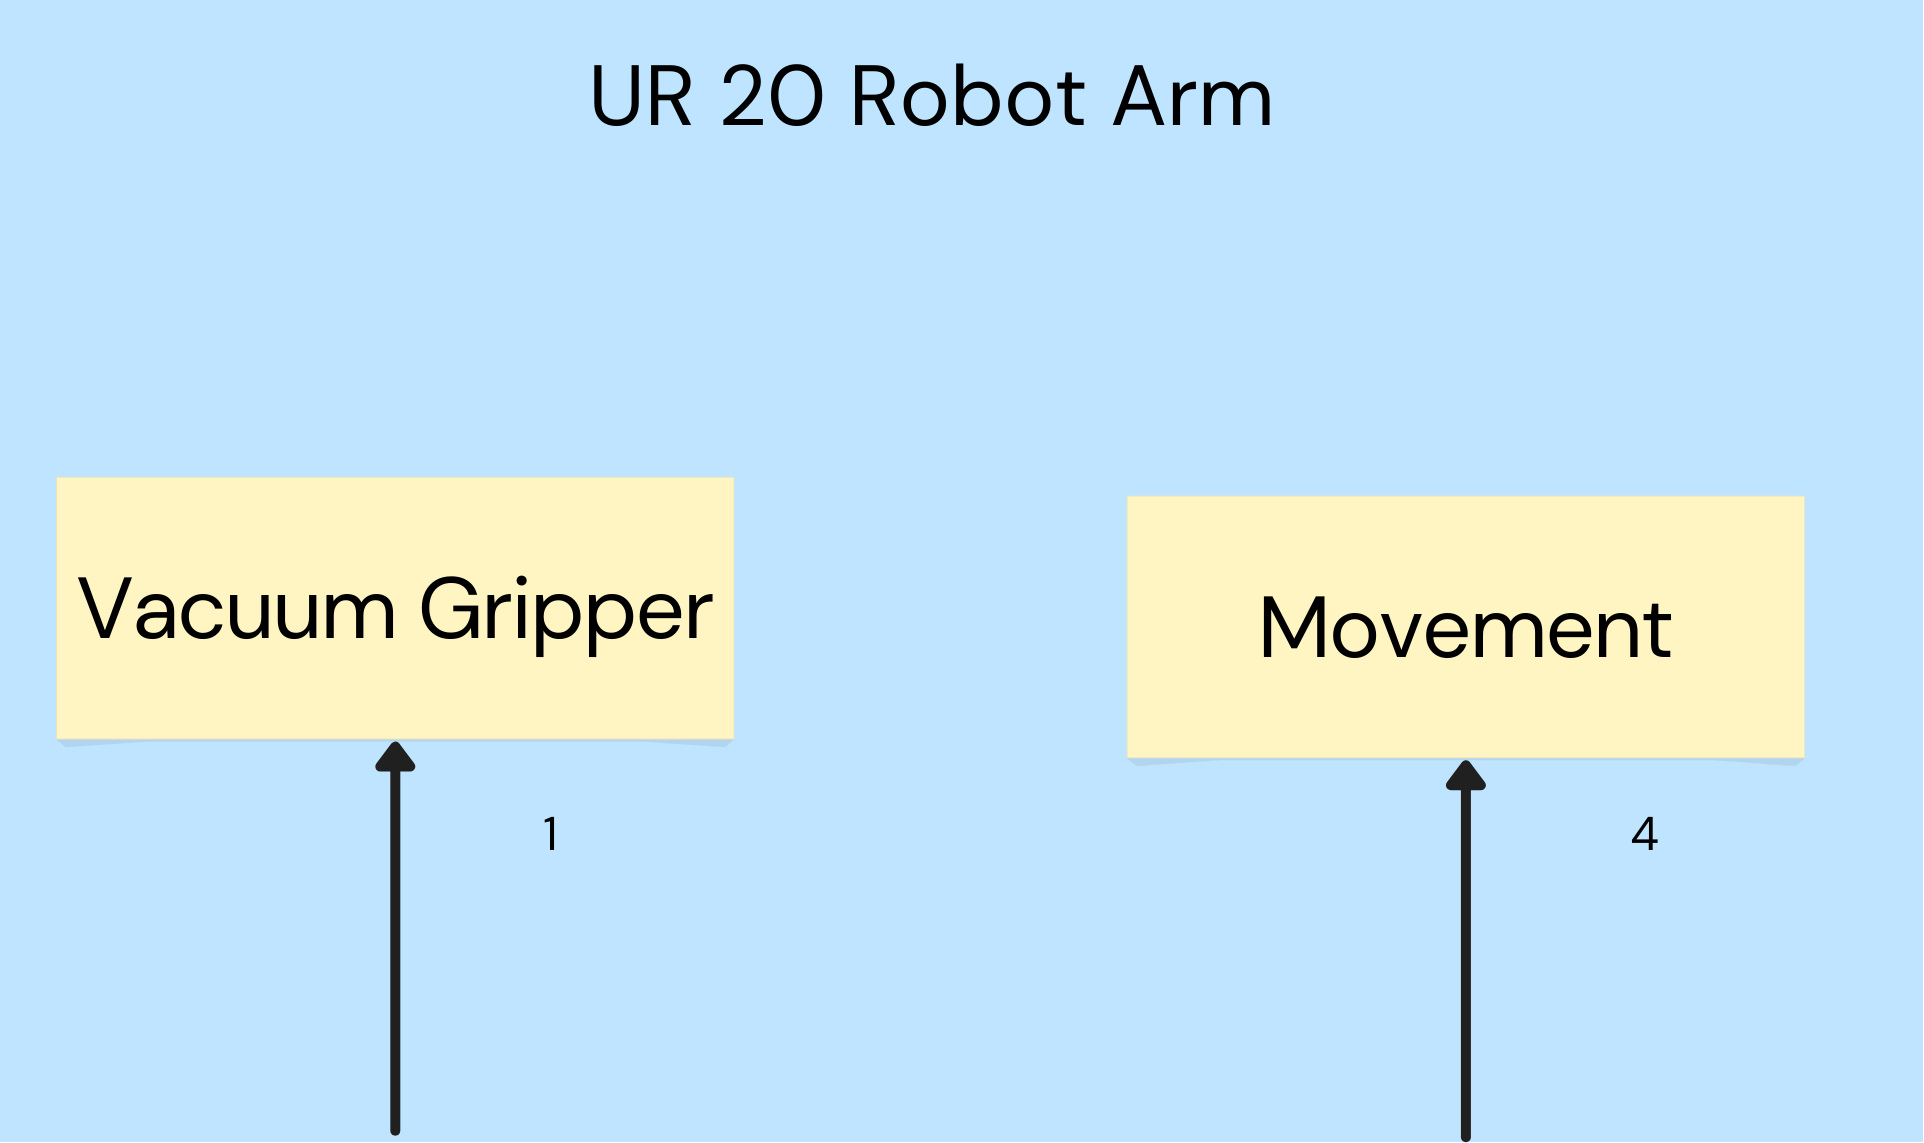
\includegraphics[width=0.60\textwidth]{images/arm}
 \caption{UR20 Arm subsystem}
\end{figure}

\subsection{Vacuum Gripper}
The Vacuum Gripper is tasked with the carrying the the incoming packages from the conveyor belt onto and releasing the package at the appropriate location on the pallet.

\subsubsection{Gripper Software Dependencies}
The Gripper will be dependent on the the voltage assignment of port (TBA) from the PLC to release and hold suction. Controlled through URScript/Python (URX library)

\subsubsection{Vacuum Hardware}
The hardware used in the gripper is the gripper itself as well as the vacuum. The gripper includes the use of an aluminum base plate, suction cups and air tube systems that connects to the vacuum. The vacuum will connect to a control box port for control.

\subsubsection{Vacuum Programming Languages}
The way to control the UR20 gripper will come from the URScript/Python

\subsection{Arm Movement}
The movement subsection of the Layer is input of the current arm location and movement of the arm to is next position whether to be in position place a box in its appropriate position or to return to the conveyor belt and await its next package.

\subsubsection{Arm Hardware}
As for the the hardware it would be the connection of the arm to its control box and control tablet access location and adjust arm position. 

\subsubsection{Arm Programming Languages}
The way to control the UR20 gripper will come from the URScript/Python

\newpage
\section{Safety Sensor Layer Subsystems}
%Jasper is doing this

The safety subsystem determines whether it is safe to continue operation (unsafe conditions are when a human is detected too close to the operation area or the emergency stop is triggered). All operations should halt when unsafe conditions are detected.

\subsubsection{Safety Sensor Programming Languages}
Python/URScript

\subsubsection{Safety Sensor Software Dependencies}
OpenCV
TensorFlow Lite
RPI.GPIO

\begin{figure}[h!]
	\centering
 	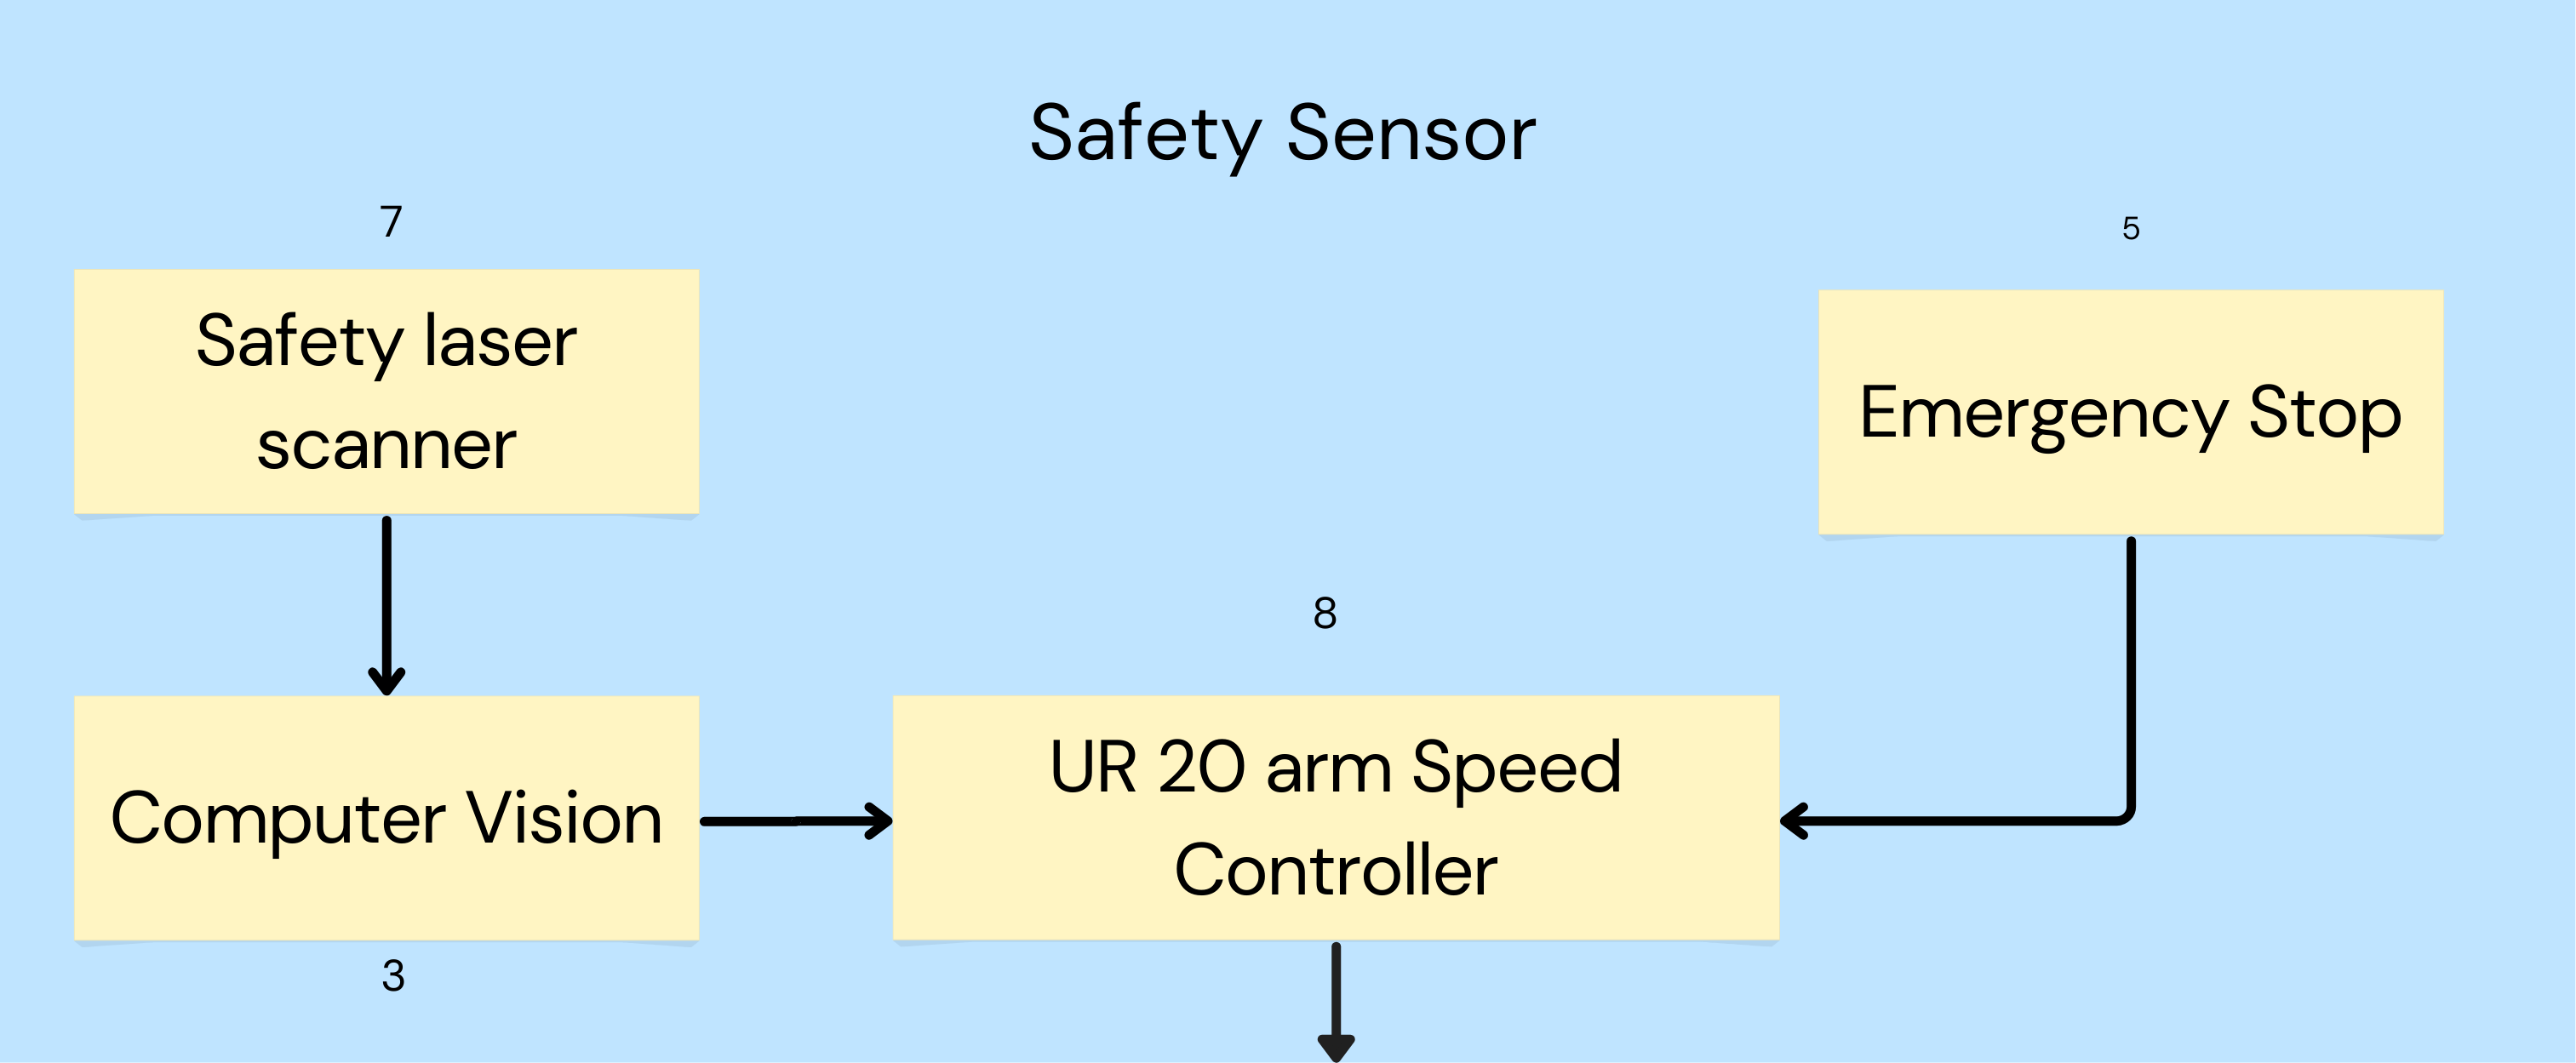
\includegraphics[width=0.60\textwidth]{images/safety.png}
 \caption{Safety sensor diagram}
\end{figure}

\subsection{Proximity Sensor Subsystem}
Detects the distance of a nearby person, if there is any person nearby.

\subsubsection{Proximity Sensor Hardware}
An IR proximity sensor mounted at the base of the robot arm, opposite the conveyor belt, detects the position and distance of any living creatures.


\subsection{Computer Vision Subsystem}
The computer vision system detectts if a human enters the operational area of the UR20 using RaspberryPi with a camera module and machine learning interface.
\subsubsection{Computer Vision Data Structures}
Input:consists of Raw image frames captured by a Raspberry Pi camera module.
Output: Classification confidence score indicating the probability of a human in dead zone of UR20 proximity sensor.

\subsubsection{Computer Vision Data Processing}
Captured frames are passed to a TensorFlow Lite model to detect humans in the frame. If the model outputs a score higher than a select threshold (0.63 in our case found through fine tuning), additional bounding box checking ensures that the detected human is within a ctritical section of the camera's view. 
If more than one person is in the dead zone, a GPIO pin is set to high, activating an emergency stop condition on the UR20.


\subsection{Speed Control Subsystem}
Determines the safest operational speed to perform at.

\subsubsection{Speed Control Data Structures}
Receives estimated distance of the nearest person from the Computer Vision subsystem.

\subsubsection{Speed Control Data Processing}
If a person is close but not within operational range, slow movement. If a person is within operational range, stop movement. Otherwise, operate at normal speed UNLESS the emergency stop is triggered, at which case ALL operation will be stopped, and if possible, manual repositioning mode will be enabled (where the arm can be moved by applying pressure).

\subsection{Emergency Stop Subsystem}
Triggers a complete stop of all operation.

\subsubsection{Proximity Sensor Hardware}
This is a physical button located on the 3PE Teach Pendant. 

\subsubsection{Proximity Sensor Data Structures}
This is integrated fully with the UR20's basic control system. A single signal will be sent to all modules that indicates whether the UR20 is controllable or in stop mode. In stop mode, no operation will be possible in any module.

\newpage
\newpage
\newpage
\section{Conveyor Belt Layer Subsystems}
The conveyor belt layer has two tasks: feed a consistent stream of boxes to the arm, and comply with safety standards. This layer has two subsystems: The ON/OFF controller, which receives signals from the PLC to start or stop the conveyor belt, and the 'Box Ready' Photo Eyes signaling system, which uses photo eyes to detect when another box is ready to be picked up.

\subsection{Conveyor Belt Hardware}
A conveyor belt provided by the Senior Design labs. 

\begin{figure}[h!]
\centering
 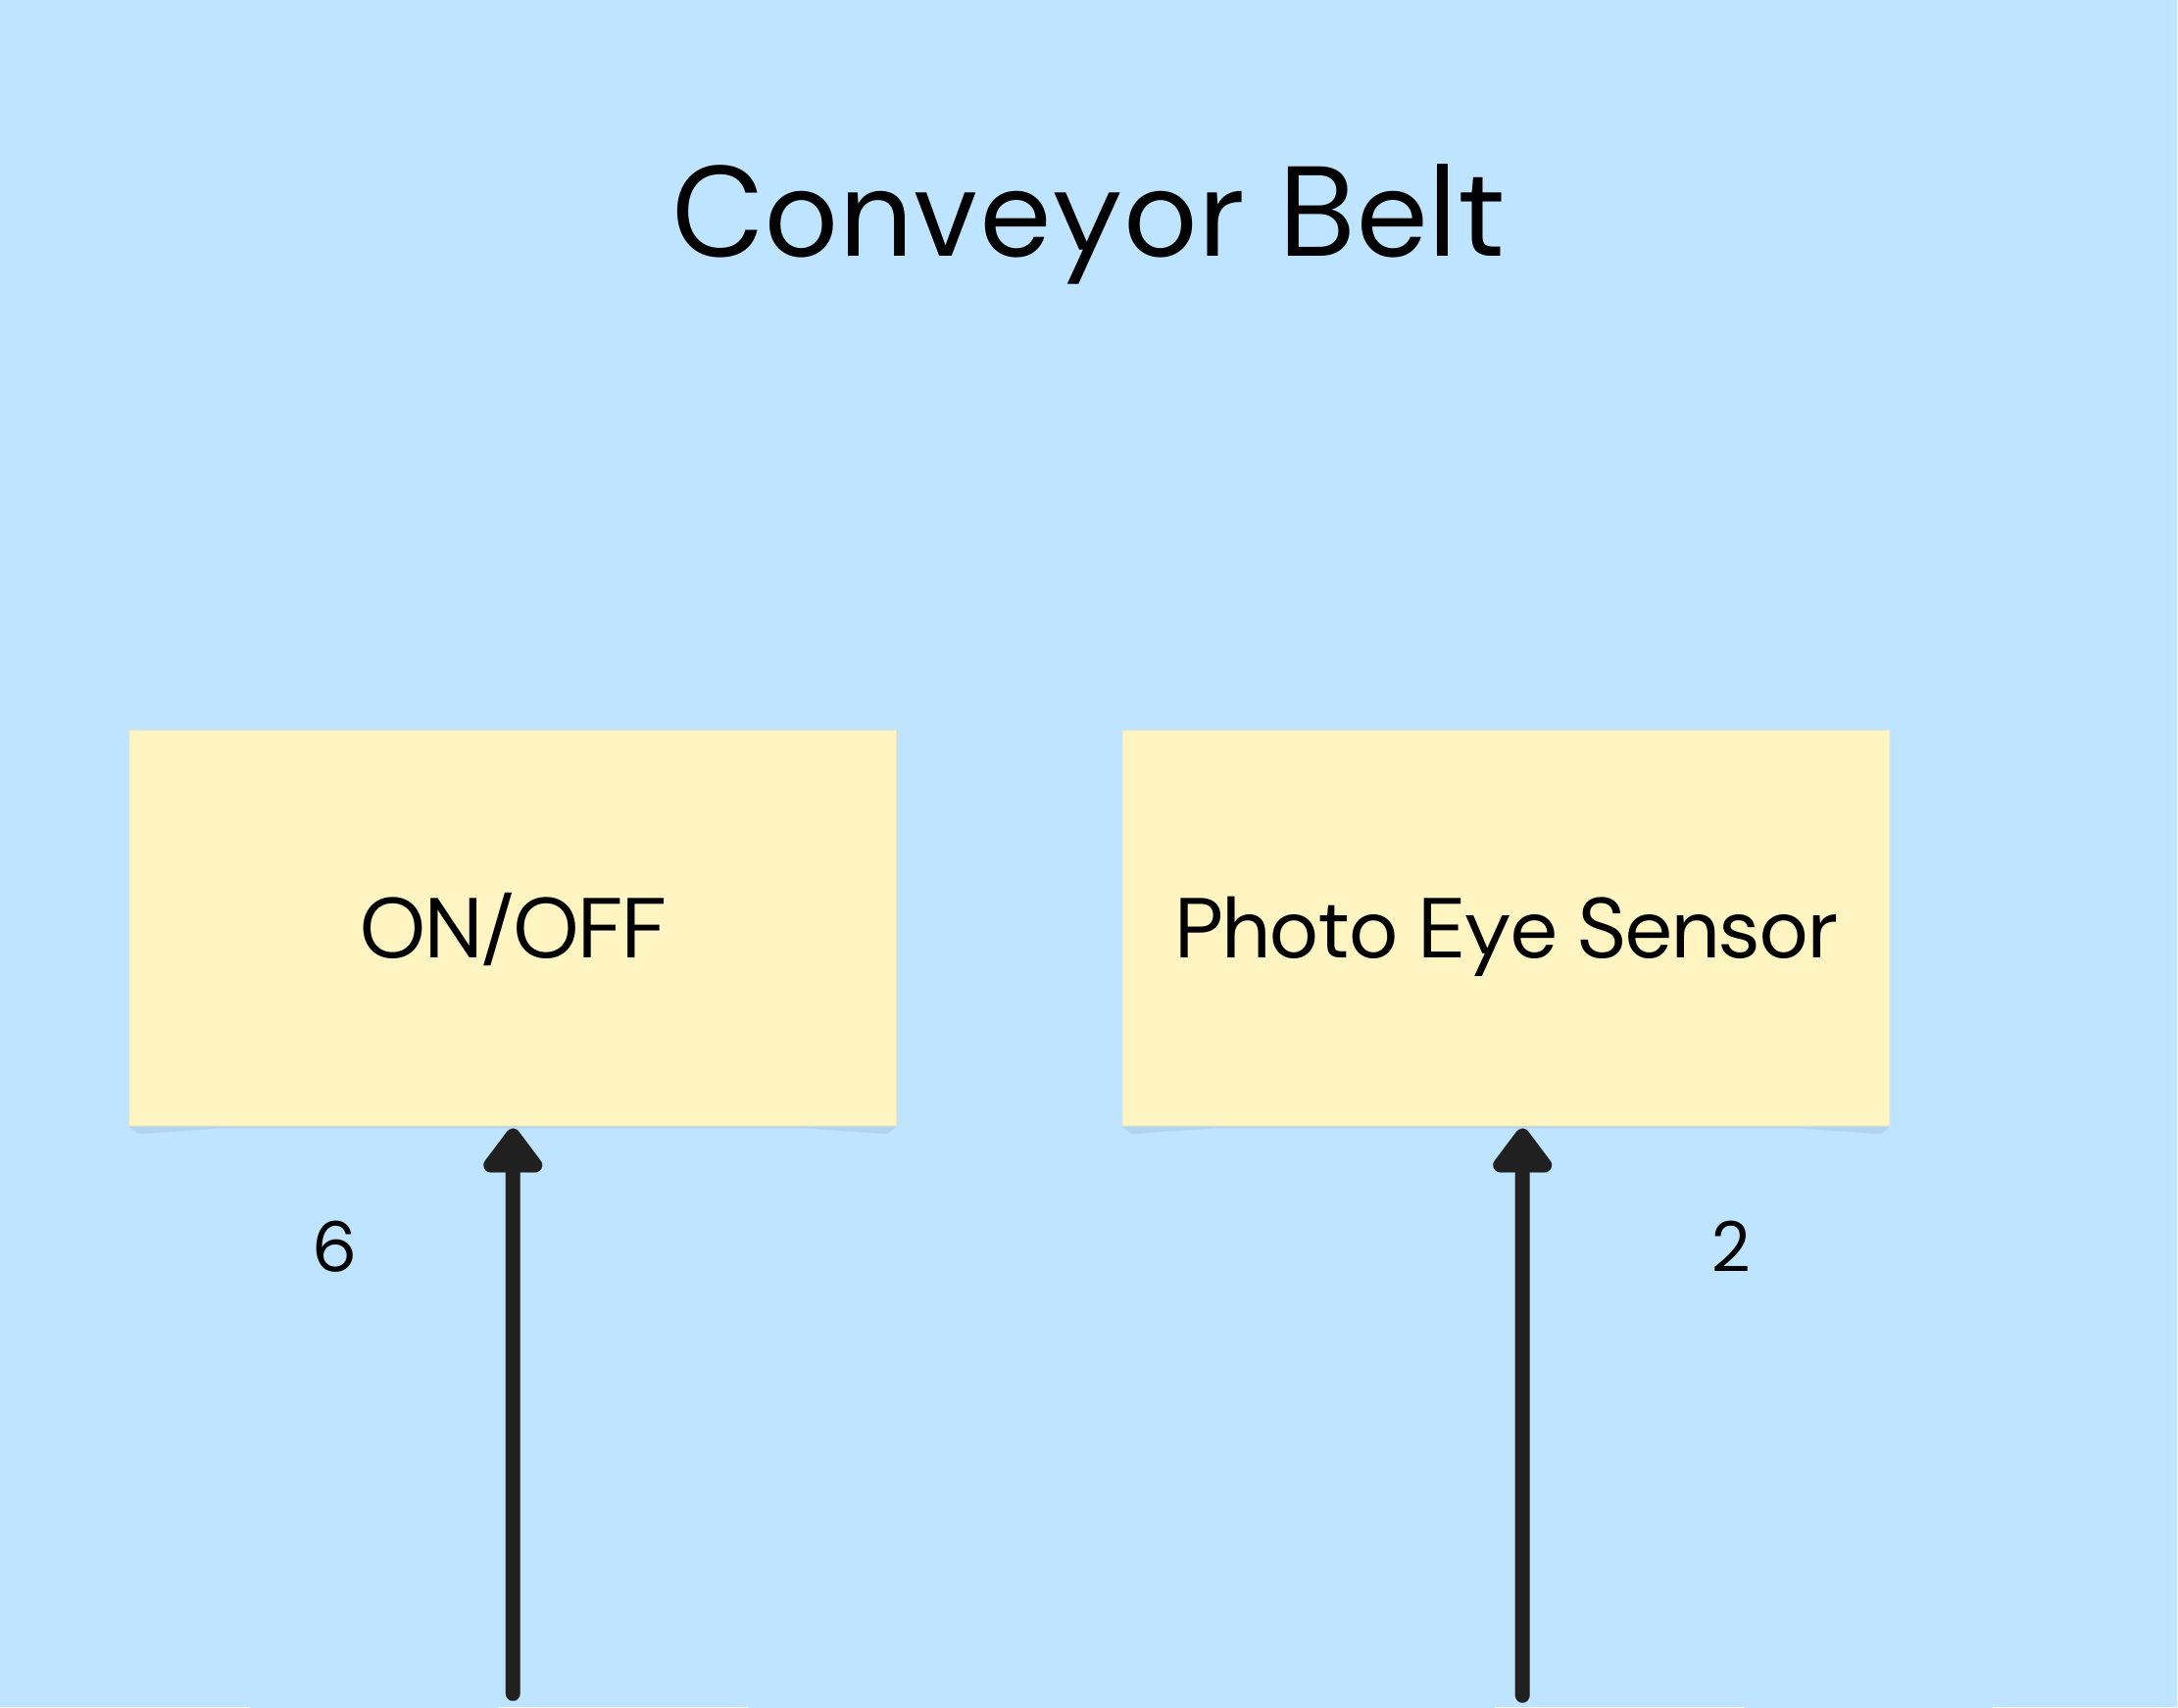
\includegraphics[width=0.60\textwidth]{images/conveyor.png}
 \caption{Conveyor belt diagram}
\end{figure}

\subsection{Power Controller Subsystem}
The power controller hardware subsystem in the conveyor belt layer is responsible for controlling the state of the conveyor belt. The subsystem receives a command from the PLC to switch the belt "ON" or "OFF" when a box moves from or into the correct position, OR when the safety system indicates an emergency stop.

\subsubsection{Power Controller Hardware}
A power supply toggle for shut-off, wired to the robot arm to be controlled by the PLA.

\subsubsection{Power Controller Data Structures}
This is a binary on/off toggle of the conveyor belt, so a single binary bit should be all that is necessary.

\subsection{Photo Eye Subsystem}
The photo eye is a simple hardware module positioned at the end of the conveyor belt to indicate that a box has passed and is ready to pick up. 

\subsubsection{Photo Eye Hardware}
Wiring between the Photo Eye and robot arm inputs.

\subsubsection{Photo Eye Data Structures}
The most common photo eye design signals use a single bit, active when presence is initially detected, and otherwise the bit signals as inactive.

\newpage
\section{PLC Layer Subsystems}
The PLC (Programmable Logic Controller) is the central control unit responsible for executing the palletizing process in a predefined sequence. It receives inputs from various sensors and controls the UR20 arm, conveyor belt, and gripper systems. The PLC is programmed to execute a routine to efficiently manage the automation cycle.
\subsection{Layer Hardware}
The PLC layer utilizes the same hardware as the subsystem which is isted below.

\subsection{Layer Operating System}
The PLC utilizes a Real-Time Operating System to ensure timely and deterministic control of hardware components.

\subsection{Box Placement Routine}

The Box Placement Routine governs the entire palletizing sequence, ensuring efficient box handling. It takes input from the safety and photo eye sensor, processes the data, and outputs commands to control the conveyor belt, vacuum gripper, and UR20 robot arm.

\begin{figure}[h!]
	\centering
 	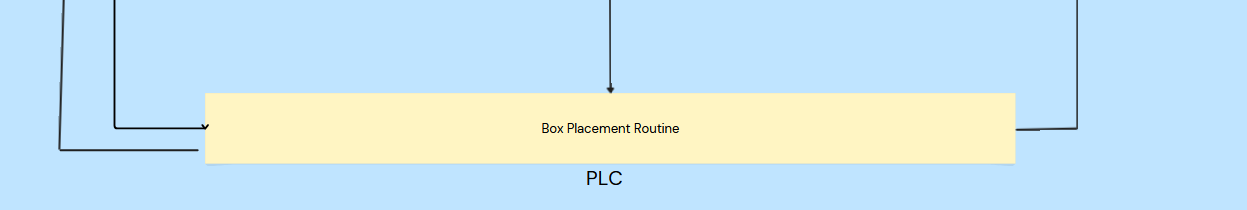
\includegraphics[width=0.60\textwidth]{images/plc.png}
 \caption{Box Placement Routine diagram}
\end{figure}

\subsubsection{Subsystem Hardware}
The Box Placement Routine subsystem utilizes the hardware from each layer as follows:
    \begin{itemize}
        \item Photo Eye Sensor: Provides input to detect boxes on the conveyor belt
        \item Safety Laser Scanner: Provides input to ensure safe operation
        \item Conveyor Belt Motor: Controlled by the PLC to turn ON/OFF
        \item Vacuum Gripper: Controlled by the PLC to pick and release boxes.
        \item UR20 Robot Arm: Moves to predefined positions for picking and placing boxes
    \end{itemize}

\subsubsection{Subsystem Operating System}
PolyScope is the software included on the 3PE Teach Pendant, utilized in setting the predefined arm movements.

\subsubsection{Subsystem Software Dependencies}
URX Python library

\subsubsection{Subsystem Programming Languages}
URSCript and Python are used to control the PLC.

\subsubsection{Subsystem Data Structures}
\begin{itemize}
    \item Sensor Data Packets:
        \begin{itemize}
            \item Photo Eye Sensor: Binary Bit (box detected or not)
            \item Safety Scanner: Binary Bit (object in range or not)
        \end{itemize}
    \item Robot Position Data: Predefined coordinates and angles for picking and placing boxes.
    \item Conveyor Belt Status: Binary Bit (ON/OFF)
    \item Vacuum Gripper Status: Binary Bit (Activated/Deactivated)
\end{itemize}

\subsubsection{Subsystem Data Processing}
The Box Placement Routine follows a state-driven algorithm, executing the following logic:
\begin{enumerate}
    \item IF Phot Eye Sensor detects a box --> STOP conveyor belt.
    \item IF safety laser scanner detects object in range of robot --> Adjust UR20 movement speed/ Halt all movement
    \item Activate vacuum gripper and move UR20 to box position
    \item Move to predefined pallet position
    \item Release vacuum gripper and return UR20 to standby position
    \item Turn conveyor belt on
    \item Repeat until palletizing sequence is complete
\end{enumerate}
\newpage





\section{Appendix A}
Include any additional documents (CAD design, circuit schematics, etc) as an appendix as necessary.
\newpage

%%% References
\bibliographystyle{plain}
%%\bibliographystyle{reference/IEEEtran_custom}
%%\bibliography{reference/refs}{}

\end{document}